\chapter{DASAR TEORI}
Pada bab ini dibahas tentang konsep yang mendasari pembahasan di bab berikutnya. Konsep dasar yang dibahas pada bab ini, yaitu konsep \textit{electric bike-sharing}, graf, proses stokastik, dan algoritma heuristik.

\section{\textit{Electric Bike-Sharing}}
Sistem \textit{electric bike-sharing} adalah salah satu bentuk transportasi berbagi (\textit{shared mobility}) di mana pengguna dapat menyewa sepeda listrik untuk perjalanan singkat di dalam kota. 

\begin{figure}[H]
    \centering
    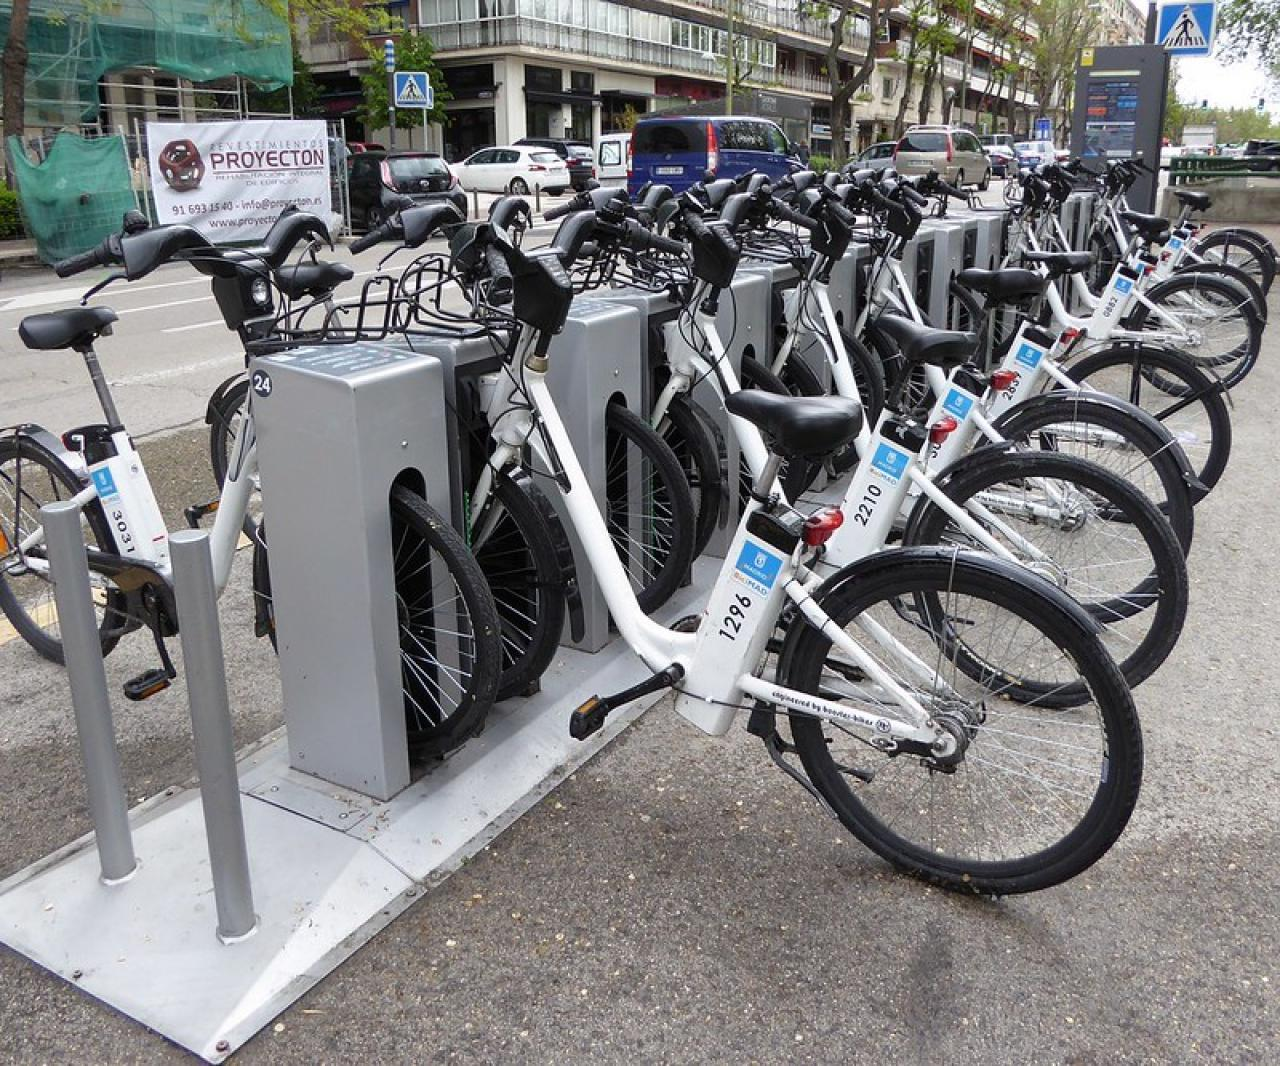
\includegraphics[scale=0.27]{Gambar FHO/e-bikes-madrid-licenced-under-cc-20-bicimad-flickr.jpg}
    \caption{Stasiun Sepeda Listrik (\protect\mycite{roadcc2021})}
    \label{Electric bike sharing}
\end{figure}

Sistem \textit{electric bike-sharing} merupakan evolusi dari sistem \textit{bike-sharing} konvensional yang menggabungkan keuntungan dari mobilitas aktif dengan teknologi \textit{electric assist} untuk memperluas jangkauan dan aksesibilitas layanan (\mycitet{fishman2020bikeshare}). Sepeda listrik dalam sistem ini umumnya dilengkapi dengan motor listrik yang membantu pengendara, terutama saat menghadapi tanjakan atau perjalanan jarak jauh, sehingga memperluas segmen pengguna potensial (\mycitet{campbell2016electric}).
Komponen kunci dari sistem \textit{electric bike-sharing} meliputi:
\begin{enumerate}
    \item \textbf{Sepeda Listrik}\\ Umumnya menggunakan sepeda dengan \textit{pedal-assist electric motor} dengan baterai yang dapat diisi ulang (\mycitet{ling2017emerging}).
    \item \textbf{Stasiun Pengisian}\\ Infrastruktur yang memungkinkan pengguna untuk mengambil dan mengembalikan sepeda serta mengisi daya baterai (\mycitet{sun2018data}).
    \item \textbf{Sistem Akses dan Pembayaran}\\ Mekanisme yang memungkinkan pengguna untuk mendaftar, membuka kunci sepeda, dan membayar layanan, biasanya melalui aplikasi smartphone atau kartu RFID (\mycitet{shaheen2019sharing}).
\end{enumerate}
Dibandingkan dengan sistem \textit{bike-sharing} konvensional, \textit{electric bike-sharing} menawarkan beberapa keunggulan:
\begin{enumerate}
    \item Dengan kemampuan sepeda listrik untuk menempuh jarak tempuh yang lebih jauh, memungkinkan pengguna untuk melakukan perjalanan yang lebih panjang (\mycitet{langford2013comparing}).
    \item Potensi untuk menggantikan perjalanan mobil jarak pendek hingga menengah yang berkontribusi pada pengurangan emisi (\mycitet{bikeplus2016shared}).
\end{enumerate}
Namun, sistem ini juga menghadapi tantangan di antaranya:
\begin{enumerate}
    \item Kebutuhan infrastruktur pengisian daya yang lebih kompleks terutama pada manajemen energi yang digunakan (\mycitet{sun2018data}).
    \item Biaya operasional yang lebih tinggi karena harga sepeda listrik dan pemeliharaan.
    \item Manajemen baterai, termasuk pengisian daya dan penggantian (\mycitet{ling2017emerging}).
\end{enumerate}
Optimalisasi lokasi stasiun pengisian daya menjadi krusial, mengingat biaya infrastruktur yang signifikan dan dampaknya terhadap aksesibilitas sistem. Model stokastik, seperti yang diusulkan oleh \mycite{brandstatter2017determining}, memungkinkan perencana untuk mempertimbangkan ketidakpastian permintaan dan variabilitas operasional dalam menentukan lokasi stasiun yang optimal.

Untuk merepresentasikan sistem \textit{bike-sharing} ini dibentuk kerangka kerja dengan menggunakan teori graf. Kerangka kerja ini dapat memodelkan konektivitas jaringan stasiun dan rute perjalanan sistem \textit{bike-sharing} dengan merepresentasikan stasiun sebagai titik dan rute trip-trip sebagai busur.

\section{Graf Berarah}
    Berikut diberikan definisi graf berarah.

\begin{definisi}
    digraf (directed graph) $G$ adalah pasangan himpunan tak kosong berhingga $V(G)$ dengan elemen-elemennya disebut titik (\textit{vertex}) dan himpunan berhingga $A(G)$ dengan elemennya merupakan pasangan berurutan $(u,v)$ dari dua titik berbeda $u$ dan $v$ di $V(G)$ yang disebut busur (arc). Pasangan himpunan titik $V(G)$ dan himpunan busur $A(G)$ dinotasikan dengan $G = (V(G), A(G))$. Untuk pasangan berurutan $(u,v)$, titik $u$ disebut titik awal dan titik $v$ disebut titik akhir dari busur tersebut.
\end{definisi}

Sebarang digraf dapat divisualisasikan dengan elemen di $V(G)$ digambarkan dalam bentuk titik/lingkaran dan elemen $(u,v)$ di $A(G)$ digambarkan sebagai busur dari $u$ ke $v$. Pada tulisan ini, penyebutan digraf akan disingkat dengan graf saja.

\begin{contoh}\label{Digraph}
    Diberikan graf seperti berikut.\\
    \begin{figure}[H]
        \centering
        \begin{tikzpicture}[scale = 0.8]
        \tikzset{vertexStyle/.append style = {shape=circle,fill=blue!10,minimum size=20pt,inner sep=1pt}}
        \Vertex[x=4.5, y=1.55,label=$C$]{C}
        \Vertex[x=3, y=0,label=$D$]{D}
        \Vertex[x=3, y=3,label=$A$]{A}
        \Vertex[x=6, y=3,label=$B$]{B}
        \Vertex[x=6, y=0,label=$E$]{E}
        \Edge[style={->}](A)(B)
        \Edge[style={->}](A)(C)
        \Edge[style={->}](D)(A)
        \Edge[style={->}](C)(E)
        \Edge[style={->}](B)(C)
        \Edge[style={->}](C)(D)
        \Edge[style={->}](B)(E) % Added arrow from E to B
        \end{tikzpicture}
        \caption{Digraf}
        \label{Digraph}
    \end{figure}

    Diperhatikan pada Gambar 2.3 terdapat digraf dengan himpunan titik yang terdiri dari $\{A,B,C,D,E\}$ dan himpunan busur yang terdiri dari $\{(A,B),(A,C),(D,A),(C,E),(B,C),(C,D),(E,B)\}$ dengan arah dalam busur ditunjukkan oleh panah. 
\end{contoh}

\begin{definisi}
     Diberikan graf $G=(V(G),A(G))$. \textit{Walk} didefinisikan sebagai barisan berhingga dari titik-titik $v_1, v_2, ..., v_m \in V(G)$ yang setiap dua titik berurutan terhubung oleh busur dan dinotasikan dengan $v_1 \rightarrow v_2 \rightarrow v_3 \rightarrow ... \rightarrow v_m$. Panjang \textit{walk} didefinisikan sebagai banyaknya busur yang dilewati dalam \textit{walk} tersebut. Selanjutnya, \textit{path} adalah \textit{walk} dengan semua titik dan busur yang dilewati berbeda. 
\end{definisi}

Untuk memperjelas perbedaan antara \textit{walk} dan \textit{path}, disajikan contoh berikut.
\begin{contoh}
    Pada Gambar \ref{Digraph} dapat dibentuk \textit{walk} $C\rightarrow D \rightarrow A \rightarrow B \rightarrow C \rightarrow E$ yang merupakan \textit{walk} dari $C$ menuju $E$ dengan panjang enam berdasarkan jumlah busur dalam \textit{walk}. Dapat dibentuk juga \textit{walk} $C \rightarrow D \rightarrow A \rightarrow B \rightarrow E$ yang merupakan \textit{path} karena titik dan busur dari \textit{walk} titik $C$ menuju titik $E$ masing-masing dilewati tepat sekali.
\end{contoh}

Dalam banyak aplikasi, termasuk dalam pemodelan sistem \textit{electric bike-sharing}, seringkali diperlukan pemberian nilai atau bobot pada busur dalam graf. Konsep ini dikenal sebagai graf berbobot yang didefinisikan sebagai berikut.
\begin{definisi}
    (\mycite{wilson1996introduction}) Bobot dari graf adalah nilai numerik yang diberikan untuk setiap busur pada graf. 
\end{definisi}

Bobot ini sering digunakan untuk merepresentasikan jarak, biaya, waktu, atau properti lain yang relevan dengan hubungan antara dua titik dalam graf. Untuk visualisasi konsep graf berbobot, disajikan contoh berikut.
\begin{contoh}
    Diberikan diagram graf seperti berikut.\\
    \begin{figure}[H]
        \centering
        \begin{tikzpicture}[scale = 0.8]
        \tikzset{vertexStyle/.append style = {shape=circle,fill=blue!10,minimum size=20pt,inner sep=1pt}}
        \Vertex[x=4.5, y=1.55,label=$C$]{C}
        \Vertex[x=3, y=0,label=$D$]{D}
        \Vertex[x=3, y=3,label=$A$]{A}
        \Vertex[x=6, y=3,label=$B$]{B}
        \Vertex[x=6, y=0,label=$E$]{E}
        \Edge[label=1,bend=0](A)(B)
        \Edge[label=2,bend=0](A)(C)
        \Edge[label=3](A)(D)
        \Edge[label=2](B)(E)
        \Edge[label=3](C)(E)
        %\Edge[bend=-15](E)(B)
        \Edge[label=1](B)(D)
        \end{tikzpicture}
        \caption{Graf Berbobot}
        \label{Graf sederhana}
    \end{figure}

    Diperhatikan pada Gambar \ref{Graf sederhana}, terdapat nilai nonnegatif, yaitu $1,2,3$ secara acak di tiap busur. Nilai-nilai tersebut adalah bobot dari graf.
\end{contoh}

Pada permasalahan stokastik lokasi stasiun pengisian daya untuk \textit{electric bike-sharing}, titik potensial pembangunan stasiun pengisian daya dapat dipandang sebagai titik. Trip tiap skenario merupakan busur, rute perjalanan dalam skenario adalah \textit{path}, kontribusi profit tiap trip merepresentasikan bobot, dan digraf merupakan arah dari trip tiap skenario (\mycite{brandstatter2017determining}).
    
\section{Program Linear Bilangan Bulat}

Program linear bilangan bulat merupakan perluasan dari program linear yang memiliki batasan tambahan pada variabel keputusannya. Sebelum membahas lebih lanjut tentang program linear bilangan bulat, penting untuk memahami konsep dasar fungsi linear dan pertidaksamaan linear.

\begin{definisi}[\mycite{winston2004operations}]
    Suatu fungsi $f: \mathbb{R}^n \rightarrow \mathbb{R}$ disebut sebagai \textbf{fungsi linear} jika dan hanya jika terdapat vektor $\boldsymbol{c} = (c_1, c_2, ..., c_n) \in \mathbb{R}^n$ sehingga untuk setiap $\boldsymbol{x} = (x_1, x_2, ..., x_n) \in \mathbb{R}^n$, berlaku
    $$f(\boldsymbol{x}) = \boldsymbol{c^T x} = {c_1x_1 + c_2x_2 + ... + c_nx_n}.$$
\end{definisi}
Untuk memperjelas konsep fungsi linear, berikut disajikan contoh fungsi linear dan bukan fungsi linear.
\begin{contoh}
    Fungsi $f(x_1,x_2)=3x_1+2x_2$ merupakan fungsi linear dari $x_1$ dan $x_2$ karena fungsi tersebut dapat ditulis dalam bentuk $c_1x_1 + c_2x_2$ dengan $c_1 = 3$ dan $c_2 = 2$.
    Sebaliknya, fungsi $f(x_1,x_2)=x_1x_2^2$ bukan merupakan fungsi linear dari $x_1$ dan $x_2$ karena fungsi tersebut mengandung perkalian antara variabel ($x_1x_2$) dan variabel berpangkat ($x_2^2$) yang tidak sesuai dengan definisi fungsi linear.
\end{contoh}

Selanjutnya, konsep pertidaksamaan linear juga penting dalam pemrograman linear. Pertidaksamaan linear didefinisikan sebagai berikut.

\begin{definisi}[\mycite{winston2004operations}]
    Diberikan fungsi linear $f: \mathbb{R}^n \rightarrow \mathbb{R}$ dan $b \in \mathbb{R}$, \textbf{pertidaksamaan linear} dapat dinyatakan dalam bentuk $f(\textbf{x}) \leq b$ atau $f(\textbf{x}) \geq b$, dengan $\textbf{x} \in \mathbb{R}^n$
\end{definisi}

Untuk lebih memahami konsep pertidaksamaan linear, diberikan contoh berikut.
\begin{contoh}
    Pertidaksamaan $x_1+4x_2\leq 3$ dan $3x_1+x_2\geq 4$ merupakan pertidaksamaan linear. Sebaliknya, $x_1^3x_2\leq 5$ bukan merupakan pertidaksamaan linear karena mengandung $x_1^3$ dan perkalian antara variabel $x_1$ dan $x_2$.
\end{contoh}

Setelah memahami konsep fungsi linear dan pertidaksamaan linear, dapat didefinisikan masalah program linear.
    \begin{definisi}[\mycite{winston2004operations}]
    Masalah program linear (LP) adalah permasalahan optimisasi dengan kriteria berikut:
    \begin{enumerate}
        \item Memaksimalkan (atau meminimalkan) fungsi linear dari variabel keputusan. Fungsi tujuan ini disebut dengan fungsi objektif.
        \item Nilai dari variabel keputusan harus memenuhi kendala. Tiap kendala berbentuk persamaan linear dan atau pertidaksamaan linear.
        \item Batasan untuk tiap variabel. Untuk setiap variabel $\boldsymbol{x}$ didefinisikan batasan secara spesifik, yaitu $x_i$ nonnegatif $(x_i\geq 0)$ untuk setiap $i=1,2,\ldots, n$ atau tidak diberi batasan.
    \end{enumerate}

    Bentuk rumusan masalah \textbf{program linear (LP)} dapat dinyatakan dalam bentuk
    \begin{align*}
        \max/\min \quad & \boldsymbol{c}^T \boldsymbol{x}, \\
        \text{dengan kendala} \quad & \boldsymbol{Ax} \leq \boldsymbol{b}, \\
        & \boldsymbol{x} \geq 0,
    \end{align*}
    dengan $\textbf{x} \in \mathbb{R}^n$ adalah vektor variabel keputusan, $\textbf{c} \in \mathbb{R}^n$ adalah vektor koefisien fungsi tujuan, $\textbf{A} \in \mathbb{R}^{m \times n}$ adalah matriks koefisien kendala, dan $\textbf{b} \in \mathbb{R}^m$ adalah vektor batas kanan kendala.
\end{definisi}

Lebih lanjut diberikan contoh masalah program linear berikut.
\begin{contoh}
    Berikut adalah contoh program linear:
    $$
    \begin{aligned}
    \text{Maksimalkan} \quad & z = 3x_1 + 2x_2, \\
    \text{dengan kendala} \quad & x_1 + x_2 \leq 10, \\
    & 2x_1 + x_2 \leq 15, \\
    & x_1, x_2 \geq 0.
    \end{aligned}
    $$
    Dalam contoh ini:
    \begin{enumerate}
        \item Tujuan  masalah di atas adalah memaksimalkan fungsi objektif $z = 3x_1 + 2x_2$ yang akan dimaksimalkan.
        \item Terdapat dua kendala: $x_1 + x_2 \leq 10$ dan $2x_1 + x_2 \leq 15$.
        \item Terdapat batasan nonnegatif pada variabel: $x_1, x_2 \geq 0$.
    \end{enumerate}
\end{contoh}

Dalam program linear, konsep daerah fisibel sangat penting. Daerah fisibel didefinisikan sebagai berikut.
\begin{definisi}[\mycite{winston2004operations}]
Daerah fisibel masalah program linear adalah himpunan dari semua titik yang memenuhi semua kendala dan batasan variabel. Daerah fisibel dapat dinyatakan sebagai berikut
$$\mathcal{F} = \{\boldsymbol{x} \in \mathbb{R}^n : \boldsymbol{Ax} \leq \boldsymbol{b}, \boldsymbol{x} \geq 0\}.$$
\end{definisi}

Untuk memvisualisasikan konsep daerah fisibel, diperhatikan contoh berikut.
\begin{contoh}
    Pada Contoh 2.3.6, daerah fisibel adalah area yang dibatasi oleh:
    \begin{enumerate}
    \item garis $x_1 + x_2 = 10$,
        \item garis $2x_1 + x_2 = 15$,
        \item sumbu $x_1$ (karena $x_2 \geq 0$), dan
        \item sumbu $x_2$ (karena $x_1 \geq 0$).
    \end{enumerate}
    Daerah ini membentuk suatu poligon dalam bidang $x_1x_2$.
    
    \begin{figure}[H]
        \centering
        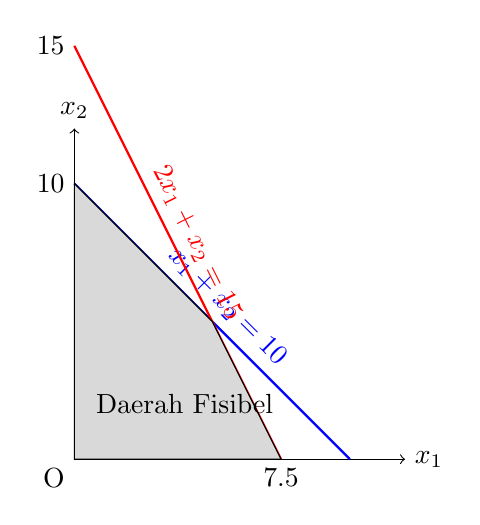
\begin{tikzpicture}[scale=0.35]
        \draw[->] (0,0) -- (12,0) node[right] {$x_1$};
        \draw[->] (0,0) -- (0,12) node[above] {$x_2$};
        \draw[thick, blue] (0,10) -- (10,0) node[midway, above, sloped] {$x_1 + x_2 = 10$};
        \draw[thick, red] (0,15) -- (7.5,0) node[midway, above, sloped] {$2x_1 + x_2 = 15$};
        
        \filldraw[fill=gray!30, draw=black] (0,0) -- (0,10) -- (5,5) -- (7.5,0) -- cycle;
        
        \node[below left] at (0,0) {O};
        \node[below] at (7.5,0) {7.5};
        \node[left] at (0,10) {10};
        \node[left] at (0,15) {15};
        
        \node at (4,2) {Daerah Fisibel};
        \end{tikzpicture}
        \caption{Daerah Fisibel untuk Contoh 2.3.6}
        \label{fig:feasible_region}
    \end{figure}
\end{contoh}

Setelah memahami daerah fisibel, dapat didefinisikan solusi optimal dari program linear.
\begin{definisi}[\mycite{winston2004operations}]
    Untuk masalah memaksimalkan, solusi optimal $\hat{x}$ dari program linear adalah
    $$\boldsymbol{\hat{x}} = \arg\max_{\boldsymbol{x} \in \mathcal{F}} \boldsymbol{c}^T \boldsymbol{x}$$
    dengan $\mathcal{F}$ adalah daerah fisibel dan $\arg\max$ (argumen maksimum) menunjukkan nilai $\boldsymbol{x}$ dalam $\mathcal{F}$ yang menghasilkan nilai maksimum dari fungsi objektif $\boldsymbol{c}^T \boldsymbol{x}$.
\end{definisi}

Untuk lebih memahami konsep solusi optimal, diperhatikan contoh berikut.
\begin{contoh}
    Dalam program linear pada contoh sebelumnya, solusi optimal akan berada pada salah satu titik sudut dari daerah fisibel. Misalkan solusi optimalnya adalah $(x_1, x_2) = (5, 5)$, maka nilai fungsi objektif maksimalnya adalah $z = 3(5) + 2(5) = 25$.
\end{contoh}

Sistem \textit{electric bike-sharing} erat berkaitan dengan program bilangan bulat karena sistem ini dibentuk dengan menentukan variabel-variabel keputusan dalam bilangan bulat seperti pembangunan stasiun potensial maupun jumlah armada sepeda yang dibutuhkan. Selanjutnya, didefinisikan program bilangan bulat.

\begin{definisi}[\mycite{winston2004operations}]
    Masalah \textbf{program bilangan bulat (IP)} adalah masalah program linear dengan tambahan kendala bahwa beberapa atau semua variabel harus berupa bilangan bulat. Bentuk umum masalah program bilangan bulat adalah
    \begin{align*}
        \max/\min \quad & \boldsymbol{c}^T \boldsymbol{x}, \\
        \text{dengan kendala} \quad & \boldsymbol{Ax} \leq \boldsymbol{b}, \\
        & \boldsymbol{x} \geq 0,\\
        & x_i \in \mathbb{Z}, \quad \text{untuk beberapa atau semua } i.
    \end{align*}
\end{definisi}

Untuk lebih memahami berbagai jenis program bilangan bulat, diperhatikan contoh berikut.
\begin{contoh}
    Berikut adalah contoh program bilangan bulat murni.
    $$\begin{aligned}
        \text{Maksimalkan} \quad & z = 3x_1 + 2x_2, \\
        \text{dengan kendala} \quad & x_1 + x_2 \leq 6, \\
        & x_1, x_2 \geq 0, \\
        & x_1, x_2 \in \Z.
    \end{aligned}$$
    Contoh program bilangan bulat campuran.
    $$\begin{aligned}
        \text{Maksimalkan} \quad & z = 3x_1 + 2x_2 ,\\
        \text{dengan kendala} \quad & x_1 + x_2 \leq 6, \\
        & x_1, x_2 \geq 0 ,\\
        & x_1 \in \Z.
    \end{aligned}$$
    Contoh IP 0-1.
    $$\begin{aligned}
        \text{Maksimalkan} \quad & z = x_1 - x_2,\\
        \text{dengan kendala} \quad & x_1 + 2x_2,\leq 2 \\
        & 2x_1 - x_2 \leq 1, \\
        & x_1, x_2 = 0 \text{ atau } 1.
    \end{aligned}$$
\end{contoh}

Dalam konteks \textit{electric bike-sharing}, program bilangan bulat dapat digunakan untuk menentukan jumlah stasiun yang harus dibangun (variabel bilangan bulat) dan kapasitas masing-masing stasiun (variabel bilangan bulat), sambil memaksimalkan cakupan layanan atau meminimalkan biaya total.

\section{Proses Stokastik dan Probabilitas}
Dalam kejadian apapun di dunia ini dapat dibedakan menjadi kepastian, ketidakpastian, dan kemustahilan. Misalkan, pasti semua sepeda listrik membutuhkan baterai untuk beroperasi,  kemungkinan orang lebih menggunakan sepeda listrik pada hari kerja, ataupun tidak mungkin sepeda listrik berubah menjadi mobil dalam perjalanan. Berdasarkan permisalan sederhana ini, dapat didefinisikan konsep \textit{randomness}.

Konsep \textit{randomness} erat kaitannya dengan probabilitas yang merupakan alat matematis untuk mengukur dan menganalisis kejadian-kejadian acak. Probabilitas memungkinkan untuk mengkuantifikasi ketidakpastian dan membuat prediksi dalam situasi yang tidak deterministik. Untuk memahami probabilitas dengan lebih baik, perlu diketahui beberapa konsep dasar (\mycite{ross2014introduction}).

% \begin{definisi} (\mycite{ross2014introduction})
%     Probabilitas adalah ukuran numerik dari kemungkinan terjadinya suatu kejadian. Nilai probabilitas berada antara 0 dan 1 dengan 0 menunjukkan kejadian yang mustahil terjadi dan 1 menunjukkan kejadian yang pasti terjadi.
% \end{definisi}

Untuk memahami bagaimana probabilitas berlaku, perlu didefinisikan ruang sampel.

\begin{definisi}(\mycite{ross2014introduction})
    Ruang sampel ($\Omega$) adalah himpunan semua hasil yang mungkin dari suatu eksperimen acak.
\end{definisi}

Setelah memahami ruang sampel, dapat didefinisikan fungsi probabilitas yang memetakan kejadian dalam ruang sampel ke nilai probabilitasnya.

\begin{definisi}
    (\mycite{billingsley1995probability}) Probabilitas $P$ adalah fungsi yang memetakan setiap kejadian $A$ dalam ruang sampel $\Omega$ ke suatu bilangan real antara 0 dan 1 yang memenuhi sifat-sifat berikut :
    \begin{enumerate}
        \item $P(A) \geq 0$ untuk setiap kejadian $A$.
        \item $P(\Omega) = 1$.
        \item Untuk kejadian-kejadian yang saling lepas $A_1, A_2, ...$, berlaku $P(\bigcup_{i=1}^{\infty} A_i) = \sum_{i=1}^{\infty} P(A_i)$.
    \end{enumerate}
\end{definisi}

Dalam program stokastik yang akan dijelaskan kemudian, erat kaitannya dengan variabel-variabel acak. Berikut didefinisikan variabel acak.

\begin{definisi}(\mycite{ross2014introduction})
    Variabel acak adalah fungsi yang memetakan setiap hasil dalam ruang sampel ke suatu bilangan real, dinotasikan dengan $X(c)=x$ dengan $c \in \Omega$ dan $x\in \mathbb{R}$
\end{definisi}

Variabel acak terbagi menjadi dua yaitu variabel acak diskrit dan variabel acak kontinu, variabel acak diskrit akan didefinisikan sebagai berikut.

\begin{definisi}(\mycite{casella2002statistical})
    Variabel acak diskrit adalah variabel acak yang hanya dapat mengambil dalam himpunan terhitung. Fungsi probabilitas dari variabel acak diskrit $X$ didefinisikan sebagai $p(x) = P(X = x)$ untuk setiap nilai $x$ yang mungkin dari $X$, dan $p(x)$ memenuhi sifat:
    \begin{enumerate}
        \item $p(x)\geq0$ untuk semua $x$,
        \item $\sum_x p(x)=1$.
    \end{enumerate}
\end{definisi}

Selanjutnya variabel acak kontinu akan didefinisikan sebagai berikut.

\begin{definisi}(\mycite{ross1996stochastic})
    Variabel acak kontinu adalah variabel acak yang dapat mengambil nilai pada suatu interval bilangan real. Variabel acak kontinu $X$ ditandai dengan fungsi kepadatan probabilitas $f(x)$, dengan probabilitas $X$ berada pada interval $[a,b]$ didefinisikan
    
    $$P(a \leq X \leq b) = \int_a^b f(x) dx,$$

    \noindent dan $f(x)$ memenuhi sifat:
    \begin{enumerate}
        \item $f(x) \geq 0$ untuk semua $x$,
        \item $\int_{-\infty}^{\infty} f(x) dx = 1$.
    \end{enumerate}
\end{definisi}

Salah satu cara untuk mendapatkan makna dari variabel-variabel acak ini adalah dengan mencari nilai ekspektasinya yang umum dalam formulasi program stokastik. Berikut didefinisikan nilai ekspektasi.

\begin{definisi}(\mycite{casella2002statistical})
    Nilai harapan atau ekspektasi dari variabel acak $X$ dengan fungsi probabilitas $p(x)$ didefinisikan sebagai
    
    \begin{align*}
        E[X] &= \sum_{x} x \cdot p(x), \quad X \text{ variabel acak diskrit}, \\
        \text{dan}\\
        E[X] &= \int x \cdot f(x) \, dx, \quad X \text{ variabel acak kontinu}.
    \end{align*}
\end{definisi}

Dalam konteks permasalahan stokastik lokasi stasiun pengisian daya untuk \textit{electric bike-sharing}, konsep probabilitas dan nilai harapan sangat penting. Permintaan pengguna sepeda listrik dapat dianggap sebagai variabel acak dan dapat digunakan nilai harapan untuk memperkirakan permintaan rata-rata pada setiap stasiun.

\begin{definisi}(\mycite{ross1996stochastic})
    Proses stokastik adalah kumpulan variabel acak $X(t)$, $t\in T$ yang diindekskan oleh parameter $t$ yang merepresentasikan waktu.
\end{definisi}

Dalam sistem \textit{electric bike-sharing}, permintaan sepeda listrik di setiap stasiun dapat dimodelkan sebagai proses stokastik yang mana permintaan bervariasi seiring waktu dan dipengaruhi oleh berbagai faktor acak seperti cuaca, hari dalam seminggu, atau acara khusus di sekitar lokasi sebagai contoh berikut.

\begin{contoh}
    Dalam sistem \textit{electric bike-sharing}, permintaan sepeda listrik di setiap stasiun dapat dimodelkan sebagai proses stokastik. Misalkan $X(t)$ mewakili jumlah permintaan sepeda listrik pada waktu $t$ di suatu stasiun tertentu. Proses stokastik ini mungkin terlihat seperti berikut.
    \begin{enumerate}
        \item $X(9:00) = 5$ (5 permintaan pada pukul 9:00),
        \item $X(10:00) = 8$ (8 permintaan pada pukul 10:00), dan
        \item $X(11:00) = 3$ (3 permintaan pada pukul 11:00).
    \end{enumerate}
\end{contoh}

Dalam pemodelan kedatangan pelanggan atau permintaan, sering digunakan distribusi Poisson. Distribusi Poisson sering digunakan untuk memodelkan kedatangan pelanggan dalam sistem antrian yang dapat diterapkan dalam konteks permintaan sepeda listrik di stasiun-stasiun pengisian daya (\mycite{grimmett2020probability}).

\begin{definisi}(\mycite{haight1967handbook})
    Distribusi Poisson adalah distribusi probabilitas diskret yang mengekspresikan probabilitas sejumlah kejadian terjadi dalam interval waktu atau ruang tertentu jika kejadian-kejadian tersebut terjadi dengan rata-rata yang diketahui dan independen terhadap waktu sejak kejadian terakhir. Fungsi massa probabilitas dari distribusi Poisson didefinisikan dengan 
    \begin{align*}
        P(X=k) = \frac{e^{-\lambda}\lambda^k}{k!}, k = 0, 1, 2, \ldots.
    \end{align*}
\end{definisi}

Selanjutnya, akan diberikan contoh dari penerapan distribusi Poisson.

\begin{contoh}
    Misalkan rata-rata kedatangan pelanggan di suatu stasiun \textit{electric bike-sharing} adalah empat orang per jam. Jika kedatangan pelanggan mengikuti distribusi Poisson, maka probabilitas tepat $k$ pelanggan datang dalam satu jam diberikan oleh
    $$P(X = k) = \frac{e^{-\lambda}\lambda^k}{k!}$$
    dengan $\lambda = 4$ (rata-rata kedatangan per jam) dan $k$ adalah jumlah kedatangan yang ingin dihitung probabilitasnya.
    Oleh karena itu, probabilitas tepat tiga pelanggan datang dalam satu jam adalah
    $$P(X = 3) = \frac{e^{-4}4^3}{3!} \approx 0.195.$$
    Ini berarti terdapat tepat tiga pelanggan akan datang dalam satu jam di stasiun tersebut dengan probababilitas sebesar 0.195.
\end{contoh}



\section{Teori Optimisasi}

Optimisasi adalah proses menemukan solusi terbaik dari suatu masalah di bawah kondisi tertentu. Dalam \textit{electric bike-sharing}, optimisasi berperan penting dalam menentukan lokasi stasiun pengisian daya yang optimal, alokasi sepeda, dan manajemen sistem secara keseluruhan. Berikut beberapa konsep utama yang relevan dalam penulisan ini.
\begin{definisi}(\mycite{nocedal2006numerical})
Diberikan masalah optimisasi
\begin{center}
    $\min_{\boldsymbol{x} \in X} f(\boldsymbol{x})$,
\end{center}
    dengan $X \subseteq \mathbb{R}^n$ adalah himpunan fisibel dan $f: X \rightarrow \mathbb{R}$ adalah fungsi tujuan. Suatu titik $\boldsymbol{x^*} \in X$ disebut solusi global jika $f(\boldsymbol{x^*}) \leq f(\boldsymbol{x})$ untuk semua $\boldsymbol{x} \in X$.
\end{definisi}
Dalam masalah penentuan lokasi stasiun pengisian daya, solusi global direpresentasikan dengan konfigurasi terbaik dari variabel keputusan sebagai contoh, konfigurasi yang dimaksud meliputi penentuan lokasi-lokasi spesifik untuk stasiun pengisian daya guna memaksimalkan keuntungan atau meminimalkan biaya secara keseluruhan.  Dalam penyelesaian model yang kompleks seperti ini dapat digunakan algoritma metaheuristik sebagai alat untuk menemukan solusi terbaik dan untuk menemukan solusi terbaik ini terlebih dahulu dicari dalam ruang pencarian.

\begin{definisi} (\mycite{glover1986future})
    Ruang pencarian $S$ adalah himpunan semua solusi yang mungkin untuk suatu masalah optimisasi. Setiap elemen $s \in S$ merepresentasikan satu konfigurasi susunan nilai variabel-variabel keputusan atau solusi potensial dari masalah yang sedang diselesaikan.
\end{definisi}

Ruang pencarian memberikan gambaran tentang semua kemungkinan solusi yang dapat dieksplorasi oleh algoritma optimisasi. Kemudian, untuk lebih memperjelas struktur ruang pencarian diperlukan fungsi \textit{neighbourhood}.

\begin{definisi} (\mycite{glover1986future})
    Fungsi neighborhood $N: S \rightarrow 2^S$ adalah fungsi yang memetakan setiap solusi $s \in S$ ke subset dari $S$ yang disebut neighborhood dari $s$. Elemen-elemen dalam $N(s)$ biasanya merupakan solusi yang dapat dicapai dari $s$ melalui modifikasi kecil atau operasi tertentu.
\end{definisi}

Berikut diberikan contoh dari fungsi \textit{neighbourhood}.

\begin{contoh}
    Misalkan sebuah sistem bike-sharing memiliki dua stasiun, masing-masing dengan kapasitas maksimal 5 sepeda. Suatu solusi direpresentasikan oleh pasangan bilangan $(x, y)$, dengan $x$ adalah jumlah sepeda di stasiun 1 dan $y$ adalah jumlah sepeda di stasiun 2.
    
    Fungsi \textit{neighborhood} $N(s)$ untuk solusi $s = (x, y)$ dapat dibentuk sebagai berikut.
    \[
    N(x, y) = \{(x', y') \mid |x' + y' - (x + y)| \leq 1, \, 0 \leq x' \leq 5, \, 0 \leq y' \leq 5\}
    \]
    \begin{enumerate}
        \item Solusi \textit{neighbor} adalah solusi yang dapat dicapai dengan memindahkan satu sepeda antar stasiun atau menambah/mengurangi satu sepeda dari sistem.
        \item Batasan $|x' + y' - (x + y)| \leq 1$ memastikan perubahan total sepeda tidak lebih dari 1.
        \item Batasan $0 \leq x' \leq 5$ dan $0 \leq y' \leq 5$ memastikan kapasitas stasiun tidak dilampaui.
    \end{enumerate}
    Diambil 2 pasangan kapasitas sepeda di stasiun 1 dan 2 sebagai berikut.
    \begin{enumerate}
        \item Jika $s = (3, 2)$, maka $N(s) = \{(2, 2), (3, 1), (3, 3), (4, 2), (2, 3), (4, 1)\}$,
        \item Jika $s = (5, 0)$, maka $N(s) = \{(4, 0), (4, 1), (5, 1)\}$.
    \end{enumerate}
\end{contoh}

Fungsi \textit{neighbourhood} ini memungkinkan algoritma optimisasi terutama metaheuristik untuk menjelajahi ruang pencarian secara efisien.

\begin{definisi} (\mycite{glover1986future})
    Metaheuristik adalah prosedur pencarian yang menggunakan strategi untuk mengeksplorasi ruang pencarian. Didefinisikan tupel $(S, f, N, M)$ dengan:
    \begin{enumerate}
    \item $S$ adalah ruang pencarian,
    \item $f: S \rightarrow \mathbb{R}$ adalah fungsi tujuan yang akan dioptimalkan,
    \item $N: S \rightarrow 2^S$ adalah fungsi neighborhood, dan
    \item $M$ adalah memori yang menyimpan informasi pencarian.
    \end{enumerate}
    Prosedur metaheuristik secara umum mencari nilai $s^* \in S$ sedemikian sehingga $f(s^*)$ optimal.
\end{definisi}

Algoritma \textit{Fire Hawk Optimizer} yang digunakan dalam penelitian ini termasuk dalam kategori metaheuristik.

\begin{contoh}
Misalkan dibentuk tupel $(S, f, N, M)$ sebagai berikut
\begin{enumerate}
    \item Himpunan $S$ adalah ruang pencarian yang terdiri dari semua konfigurasi yang mungkin untuk penempatan stasiun dan alokasi sepeda. Misalnya, $\boldsymbol{s} \in S$ mungkin direpresentasikan sebagai vektor $\boldsymbol{s} = (x_1, ..., x_n, y_1, ..., y_n)$, dengan $x_i$ adalah lokasi stasiun ke-$i$ dan $y_i$ adalah jumlah sepeda di stasiun tersebut.
    
    \item Fungsi $f: S \rightarrow \mathbb{R}$, merepresentasikan total keuntungan yang dinyatakan dalam 
    $$f(\boldsymbol{s}) = \sum_{i=1}^n (p_i y_i - c_i x_i) - \sum_{u \in U} \alpha_u d_u(\boldsymbol{s})$$
    dengan $p_i$ adalah profit per sepeda di stasiun $i$, $c_i$ adalah biaya pembangunan stasiun $i$, $\alpha_u$ adalah probabilitas skenario permintaan $u$, dan $d_u(\boldsymbol{s})$ adalah fungsi yang mengukur ketidakpuasan permintaan untuk konfigurasi $\boldsymbol{s}$ dalam skenario $u$.
    
    \item Fungsi $N: S \rightarrow 2^S$ adalah fungsi neighborhood yang mendefinisikan solusi-solusi yang dapat dicapai dari suatu solusi dengan modifikasi. Misalnya,
    \begin{align*}
        N(\boldsymbol{s}) = \{\boldsymbol{s'} \in S \mid \boldsymbol{s'} \text{ didapat dengan memilih stasiun} \\
        \phantom{N(s) = \{s' \in S \mid} \text{atau mengubah alokasi sepeda}\}
    \end{align*}
    
    \item Notasi $M$ merupakan struktur memori yang menyimpan informasi pencarian, seperti solusi terbaik yang ditemukan sejauh ini, frekuensi pencarian ke area tertentu dalam ruang pencarian, atau tren perubahan fungsi tujuan.
\end{enumerate}

Tujuan dari metaheuristik ini adalah menemukan nilai $\boldsymbol{s^*} \in S$ yang memaksimalkan $f(\boldsymbol{s})$. Seperti halnya algoritma \textit{fire hawk optimizer} terdiri dari struktur ini untuk mengeksplorasi ruang pencarian $S$, mengevaluasi solusi $f$, menggunakan $N$ untuk bergerak antar solusi, dan memanfaatkan $M$ untuk menyimpan dan menggunakan informasi selama proses pencarian.

\end{contoh}
